%% Artigo da dissertacao — modelo Elsevier (elsarticle), fornecido pelo Prof. Luis Nunes.
%% Versao destilada da dissertacao "Aprendizagem por Reforco para Controlo de Enxames".
\documentclass[final,5p,times,twocolumn,authoryear]{elsarticle}

\usepackage[T1]{fontenc}
\usepackage[utf8]{inputenc}
\usepackage[portuguese]{babel}
\usepackage{amsmath}
\usepackage{amssymb}
\usepackage{booktabs}
\usepackage{graphicx}
\usepackage{url}

\journal{Pré-publicação --- ISCTE-IUL / ISTAR}

\begin{document}

\begin{frontmatter}

\title{Aprendizagem Adaptativa \emph{versus} Robustez Estática: Comparação de
Aprendizagem por Reforço e Neuroevolução para Controlo de Enxames}

\author[iscte]{Gon\c{c}alo Pombo}
\ead{goncalopombo123@gmail.com}
\author[iscte]{Lu\'is Nunes}

\affiliation[iscte]{organization={Instituto Universit\'ario de Lisboa (ISCTE-IUL), ISTAR},
            city={Lisboa},
            country={Portugal}}

\begin{abstract}
O controlo de enxames robóticos é abordado por duas comunidades que raramente se
encontram num referencial comum: a aprendizagem por reforço multiagente (MARL),
que promete adaptabilidade \emph{em linha}, e a otimização bio-inspirada, que
oferece robustez pré-programada. Este trabalho apresenta uma comparação
controlada e independente do paradigma entre três controladores --- uma rede de
grafo neuroevoluída com atenção sobre os vizinhos, \emph{Proximal Policy
Optimisation} (PPO) e \emph{Soft Actor--Critic} (SAC) --- no mesmo simulador
tridimensional de \emph{foraging} de alta fidelidade, com seis cenários de
dificuldade crescente, sob avaliação determinística e testes estatísticos. Na
realização da tarefa, os métodos de gradiente dominam: o SAC resolve os seis
cenários e o PPO cinco em seis, falhando o Muro~em~U por \emph{exploração da
recompensa} (\emph{reward hacking}), ao passo que o controlador evolutivo colapsa
nos cenários com estrangulamentos. O quadro inverte-se sob escalabilidade
\emph{zero-shot}: apenas o controlador baseado em atenção transita de $N=10$ para
$N=100$ agentes sem retreino, uma vez que as políticas de dimensão fixa do
PPO/SAC são estruturalmente incompatíveis com $N\neq 20$. A hipótese de que a
inteligência adaptativa domina a robustez estática é, por isso, apenas
\emph{parcialmente} confirmada, revelando um compromisso central entre o
desempenho na tarefa a um tamanho de enxame fixo e a escalabilidade para tamanhos
nunca vistos.
\end{abstract}

\begin{keyword}
robótica de enxames \sep aprendizagem por reforço multiagente \sep neuroevolução
\sep escalabilidade zero-shot \sep redes neuronais de grafos \sep avaliação comparativa
\end{keyword}

\end{frontmatter}

\section{Introdução}
\label{sec:intro}
Os enxames robóticos prometem soluções escaláveis e resilientes para tarefas como
busca e salvamento, monitorização ambiental e logística distribuída. A questão
central de engenharia é qual o paradigma de controlo que melhor mantém a
operacionalidade sob incerteza. Duas escolas dominam. A \emph{otimização
bio-inspirada} (por exemplo, algoritmos evolutivos e otimização por enxame de
partículas) procura num espaço global de parâmetros, \emph{fora de linha},
controladores robustos e estáticos \citep{kennedy1995pso}. A \emph{aprendizagem
por reforço multiagente} (MARL) aprende, em alternativa, políticas adaptativas
\emph{em linha} através da interação \citep{huh2023marl}. Apesar do extenso
trabalho em cada uma, as comparações diretas e rigorosas entre paradigmas
permanecem escassas \citep{majid2023deep, bettini2024benchmarl}: os estudos
costumam refinar um único algoritmo contra variantes da sua própria família,
descurando as referências cruzadas entre paradigmas.

Controlar um enxame é difícil por três razões que se reforçam. O espaço de ações
conjuntas cresce exponencialmente com o número de agentes, tornando inviável tratar
o enxame como um único agente monolítico; a recompensa de tarefa é tipicamente
esparsa e diferida, o que agrava a atribuição de crédito; e cada agente decide a
partir de uma observação parcial e local, sem acesso ao estado global. Os dois
paradigmas respondem a estas dificuldades de formas opostas --- a MARL aprende uma
política partilhada que generaliza por experiência, a otimização bio-inspirada
procura um controlador robusto num só esforço de otimização --- e é precisamente
essa oposição que motiva uma comparação direta e controlada.

A questão de investigação que orienta a dissertação é, em rigor, se a
\emph{inteligência adaptativa} (uma política de MARL que aprende com a
experiência) supera a \emph{robustez estática} (um controlador otimizado de uma
só vez e depois congelado) em cenários de \emph{stress} dinâmico. Responder a
esta questão exige um referencial em que ambos os paradigmas sejam avaliados nas
mesmas condições, com as mesmas métricas e a mesma análise estatística --- algo
que a literatura raramente oferece.

Este artigo aborda essa lacuna com uma avaliação comparativa imparcial.
Implementámos um simulador tridimensional de \emph{foraging} de alta fidelidade e
avaliámos três controladores --- uma rede de grafo neuroevoluída com
auto-atenção sobre os vizinhos, PPO e SAC --- em seis cenários, ao longo de três
eixos: desempenho na tarefa ($P_{\text{task}}$), robustez a falhas de agentes
($R_{\text{robust}}$) e escalabilidade \emph{zero-shot} ($S_{\text{scale}}$),
todos suportados por testes de significância não paramétricos. A nossa
contribuição é dupla: (i) um protocolo de avaliação reprodutível e independente
do paradigma; e (ii) a evidência de um compromisso central, em que os métodos de
gradiente vencem na realização da tarefa a um tamanho de enxame fixo, enquanto
apenas o controlador baseado em grafo escala para tamanhos de enxame nunca
vistos. A metodologia e os resultados completos são detalhados na dissertação que
acompanha este artigo.

\section{Trabalho Relacionado}
\label{sec:related}
A aprendizagem por reforço profunda tem sido aplicada a sistemas de enxame com
partilha de parâmetros para domar a explosão do espaço de ações conjuntas
\citep{huttenrauch2019deep}, em que uma única rede é partilhada por todos os
agentes homogéneos. As redes neuronais de grafos (GNN) emergiram como o principal
viabilizador da escalabilidade: ao modelar o enxame como um grafo e ao aplicar
atenção sobre os vizinhos, uma política treinada com poucos agentes pode ser
implantada com muitos \citep{sun2024graph}. O mecanismo de atenção
\citep{vaswani2017attention, velickovic2018gat} é central nesta propriedade, por
ser invariante à permutação e à cardinalidade do conjunto de vizinhos. Os
controlos de enxames baseados em grafos têm-se multiplicado, com aplicações que
vão da estimação distribuída em redes dinâmicas \citep{sun2024graph} ao controlo
descentralizado de formação \citep{schmickl2025gnn, elrod2025gnn}, e revisões
recentes consolidam a GNN como o substrato dominante para a escalabilidade em
enxames \citep{lin2025survey}.

No paradigma de aprendizagem, o esquema de treino centralizado com execução
descentralizada (CTDE) tornou-se padrão para domar a não-estacionariedade do
ambiente multiagente \citep{lowe2017maddpg, oliehoek2016concise}. No presente
trabalho, contudo, os \emph{baselines} de gradiente partilham uma única política
e executam a partir da observação puramente local, sem um crítico de estado
global, o que mantém a comparação ancorada num regime descentralizado comum aos
três controladores.

Do lado bio-inspirado, a neuroevolução otimiza os pesos da rede sem gradientes
\citep{salimans2017es}, oferecendo controladores estáveis para tarefas estáticas,
mas com adaptabilidade \emph{em linha} limitada \citep{kegeleirs2025towards}. As
estratégias de evolução são atrativas pela simplicidade e pela
paralelização trivial, mas otimizam a partir de um único escalar de aptidão por
episódio, sem atribuição de crédito temporal --- uma distinção que se revelará
decisiva nos resultados.

Os estudos comparativos entre aprendizagem por reforço profunda e estratégias de
evolução salientam a ausência de uma referência de desempenho comum entre as duas
famílias \citep{majid2023deep}, enquanto os referenciais padronizados de MARL
permanecem focados dentro da comunidade de aprendizagem \citep{bettini2024benchmarl}.
As aplicações de aprendizagem por reforço profunda à navegação de enxames
\citep{iskandar2023navigation} ilustram o tipo de estudo de paradigma único que
este trabalho estende, com uma comparação sistemática e estatisticamente
fundamentada contra a alternativa bio-inspirada.

\section{Metodologia}
\label{sec:method}

\subsection{Ambiente de simulação}
O ambiente é uma tarefa de \emph{foraging} contínua e tridimensional, numa arena
circular (raio $15$\,m) com $N=20$ agentes homogéneos que devem recolher comida e
transportá-la para um ninho. Utilizam-se seis cenários de dificuldade crescente:
um \emph{Sandbox} aberto; três labirintos de navegação (\emph{Muro em U},
\emph{Gargalo}, \emph{Quatro Salas}); e duas tarefas cooperativas (\emph{Porta
Cooperativa}, que exige $\geq 3$ agentes para abrir uma passagem, e \emph{Perceção
Cooperativa}, com um alvo móvel). A Figura~\ref{fig:mapas} ilustra os seis
cenários. Cada agente observa uma bússola de \emph{homing} egocêntrica para o
ninho, oito raios LiDAR para deteção local de obstáculos e o estado relativo dos
vizinhos --- um cenário parcialmente observável, formalizável como um Dec-POMDP
\citep{oliehoek2016concise}. A bússola fornece a direção e a distância euclidiana
ao ninho de forma sempre disponível (à imagem do \emph{homing} global em formigas
ou da navegação por GPS), ao passo que os obstáculos só são percecionados
localmente pelo LiDAR de $5$\,m, preservando uma observabilidade parcial genuína.

\begin{figure*}[t]
\centering
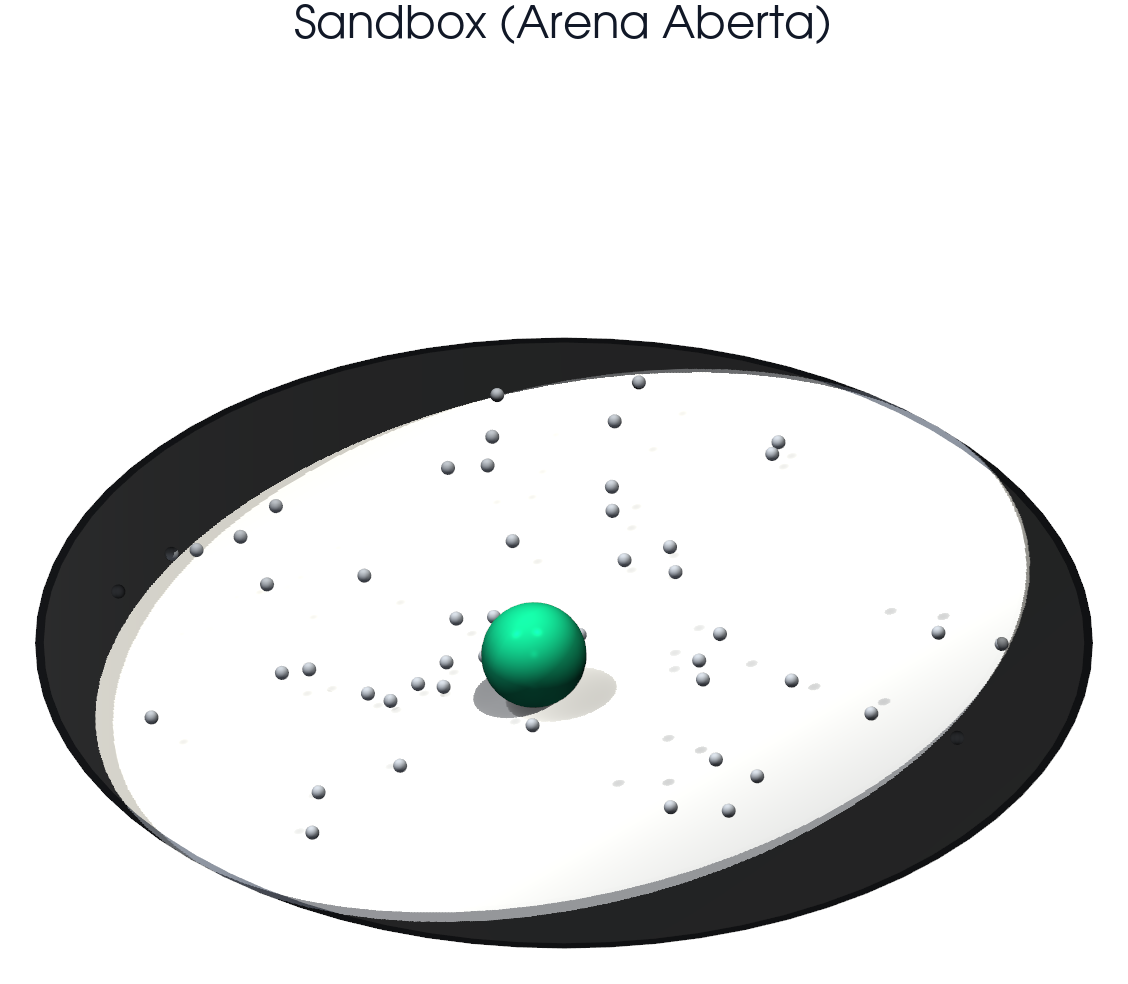
\includegraphics[width=0.32\linewidth]{images/mapa_3d_none.png}\hfill
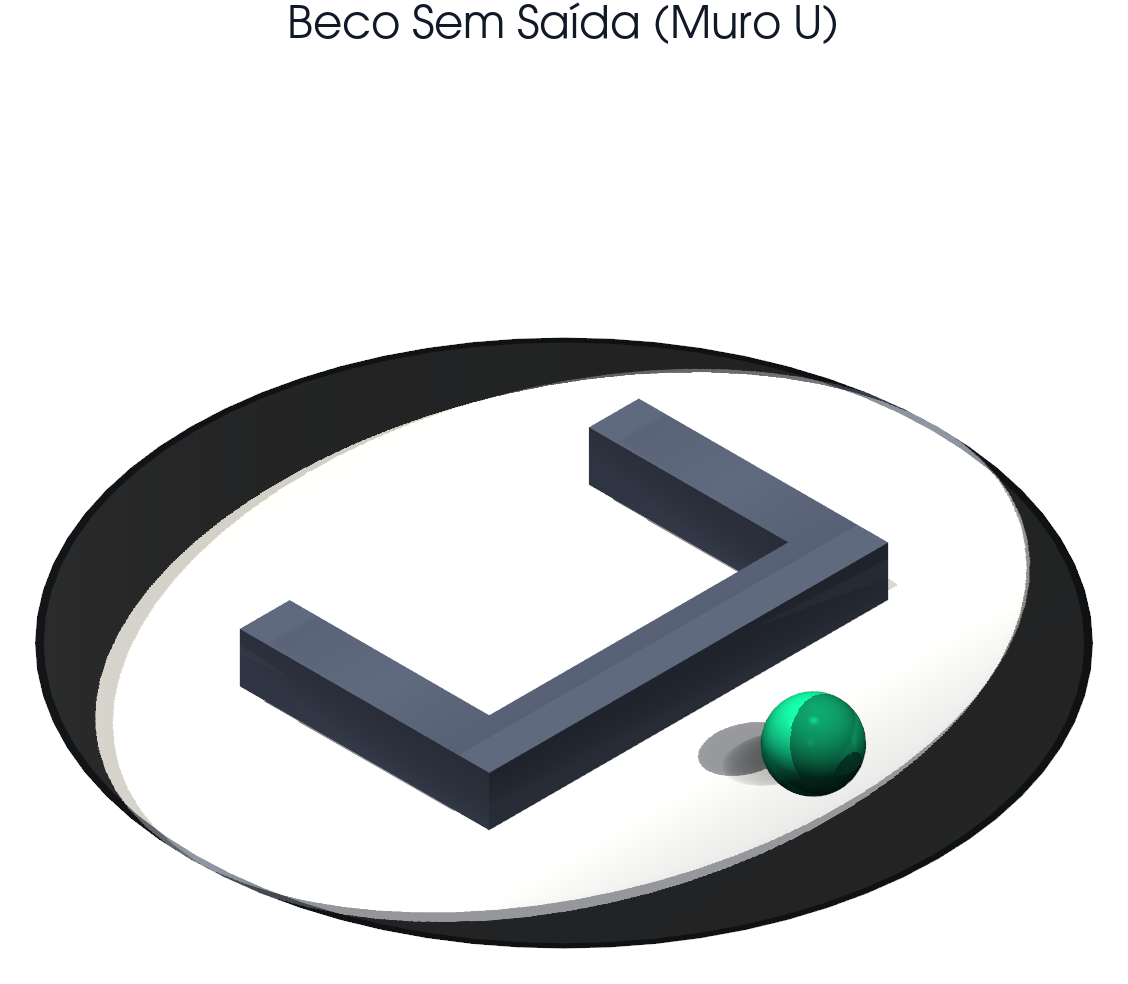
\includegraphics[width=0.32\linewidth]{images/mapa_3d_u_wall.png}\hfill
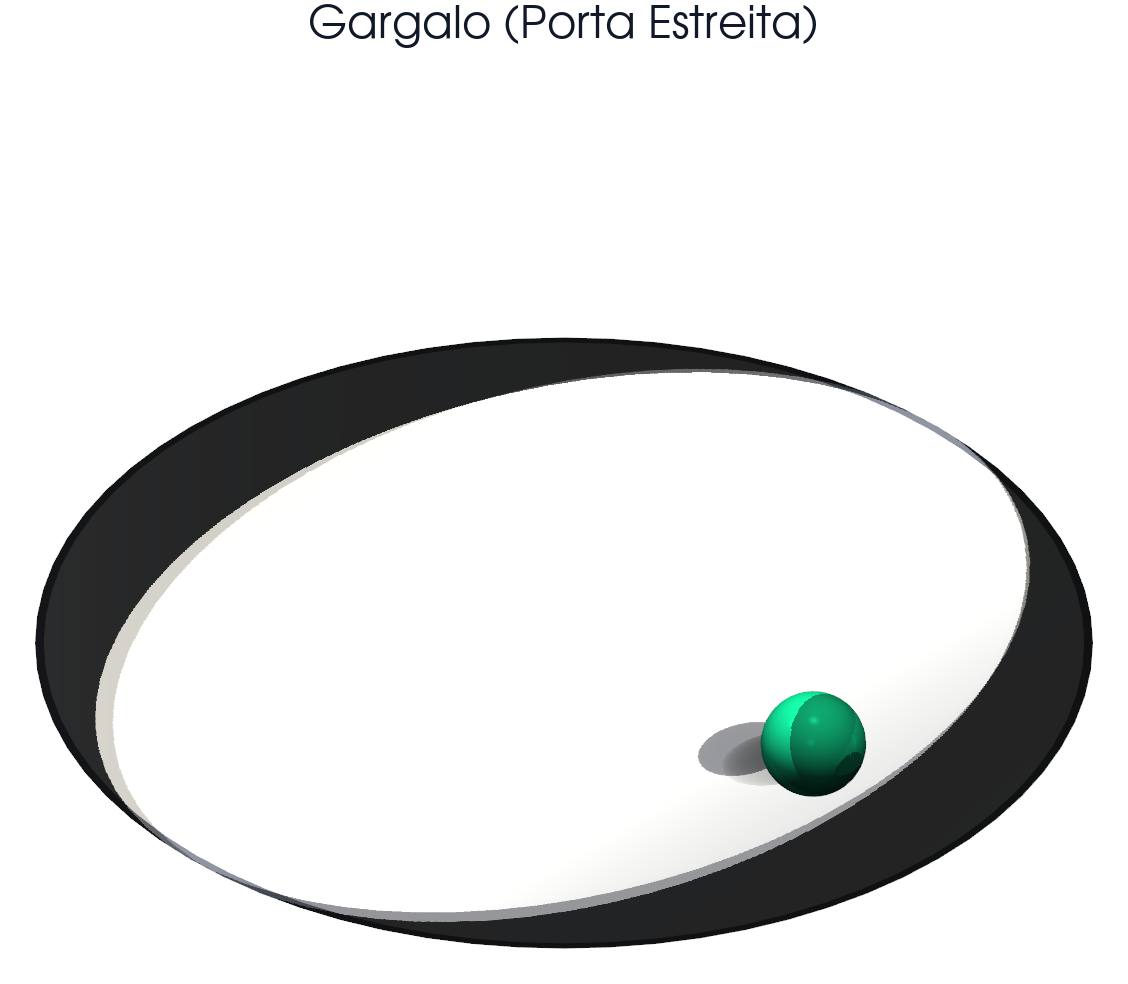
\includegraphics[width=0.32\linewidth]{images/mapa_3d_bottleneck.png}\\[2pt]
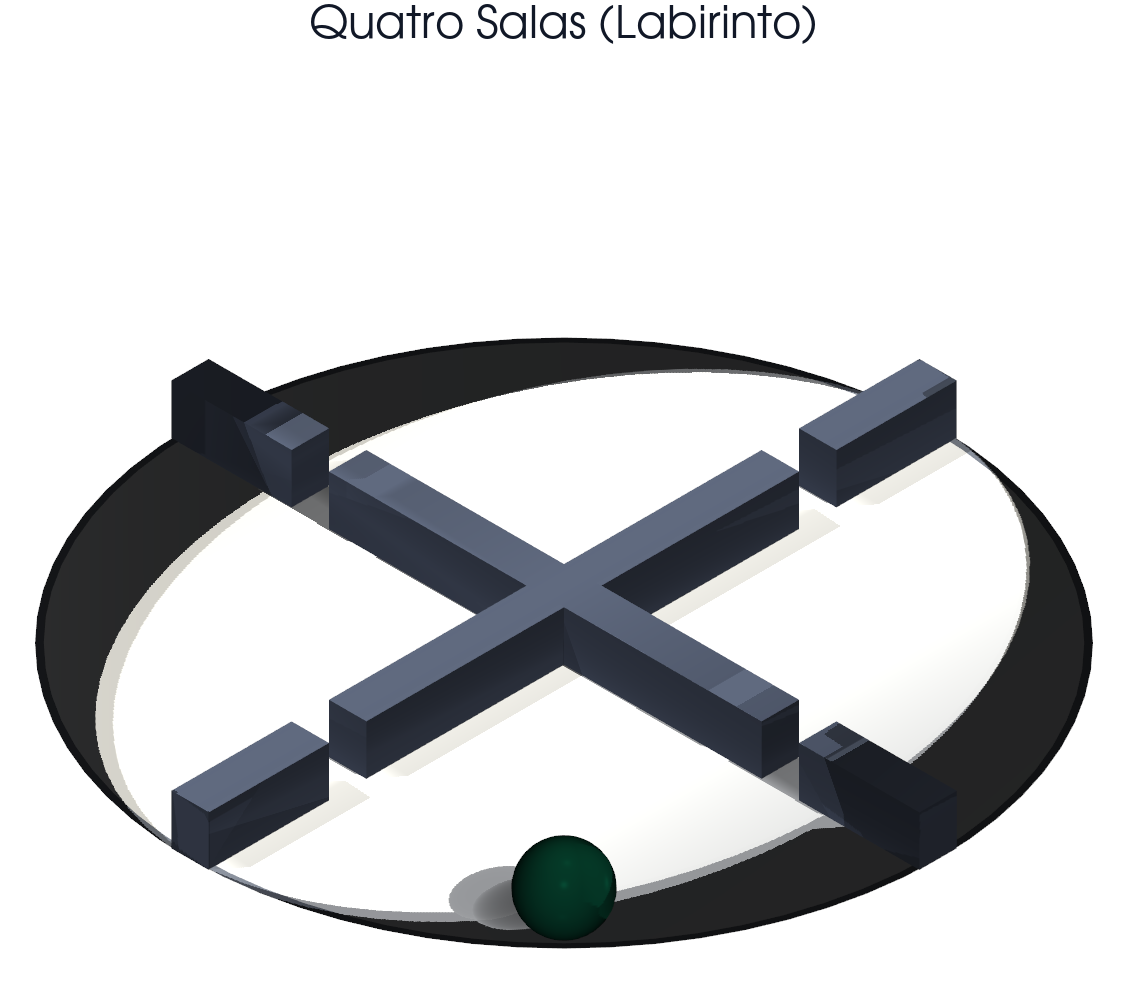
\includegraphics[width=0.32\linewidth]{images/mapa_3d_four_rooms.png}\hfill
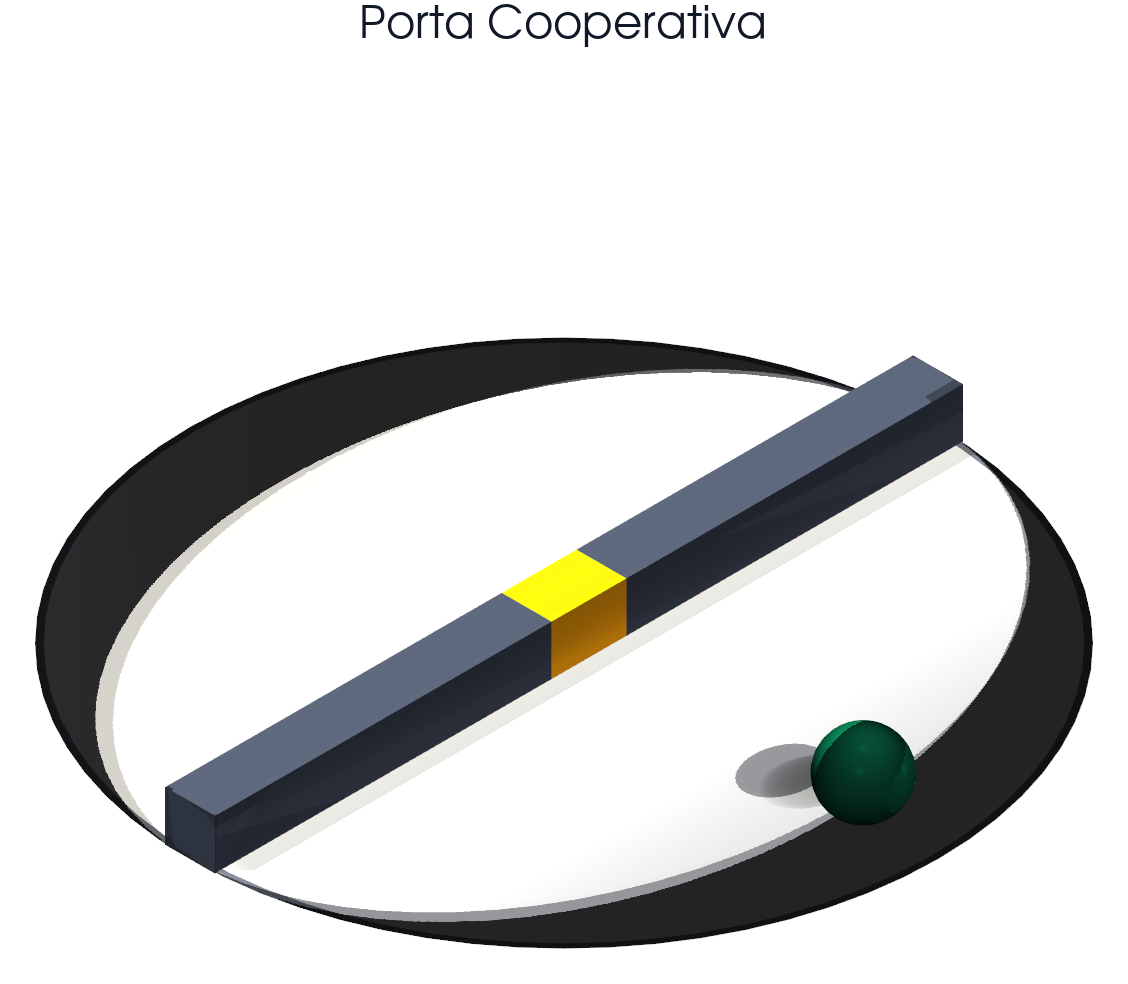
\includegraphics[width=0.32\linewidth]{images/mapa_3d_cooperative_door.png}\hfill
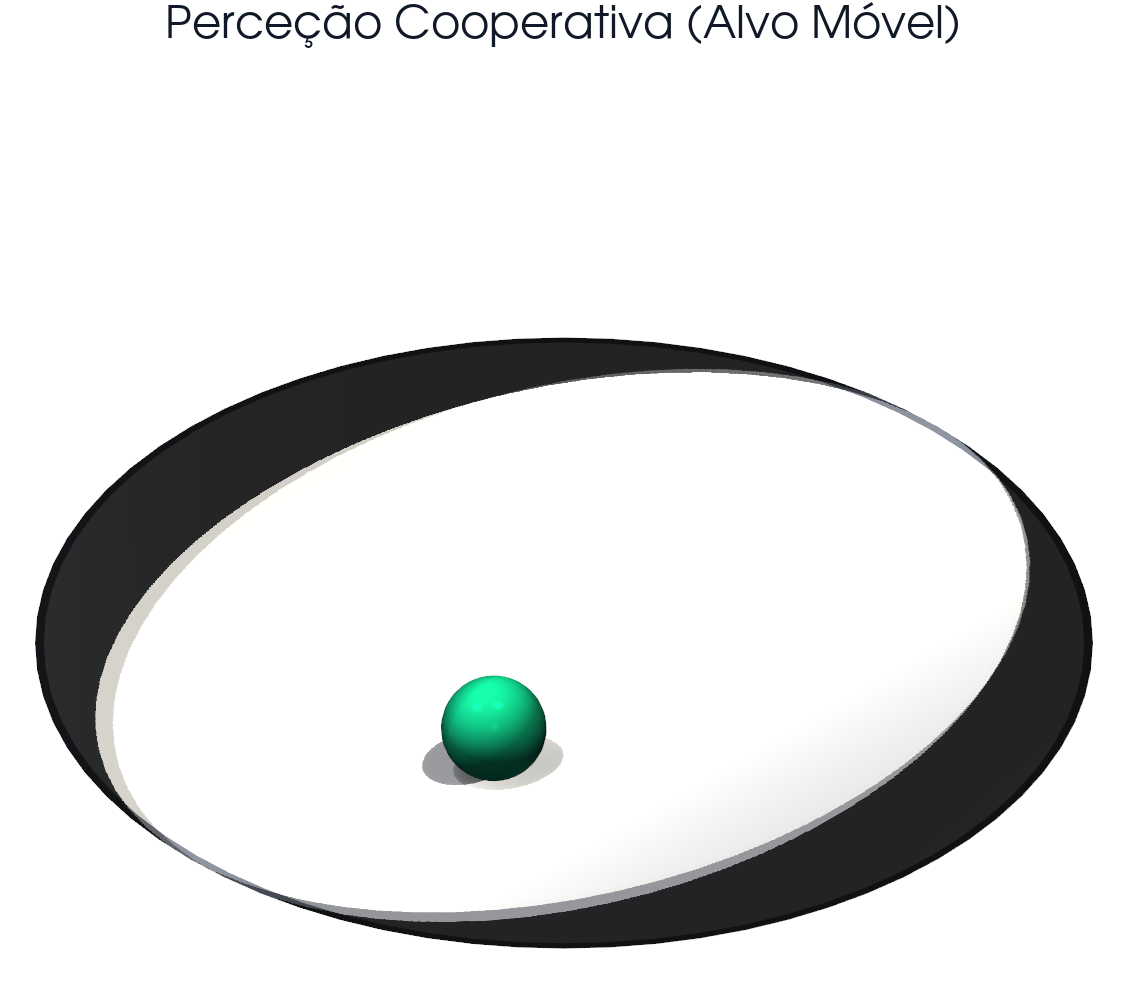
\includegraphics[width=0.32\linewidth]{images/mapa_3d_cooperative_perception.png}
\caption{Os seis cenários de avaliação, renderizados a partir da geometria real
do simulador. Em cima: Sandbox (aberto, com obstáculos esféricos), Muro em U e
Gargalo. Em baixo: Quatro Salas, Porta Cooperativa (passagem a âmbar, abre com
$\geq 3$ agentes) e Perceção Cooperativa (alvo móvel). O ninho é a esfera verde.}
\label{fig:mapas}
\end{figure*}

Para evitar mínimos locais nos cenários de labirinto, a recompensa de progresso
usa um potencial \emph{geodésico} calculado pelo algoritmo de Dijkstra sobre uma
grelha de ocupação dilatada, atuando como modelação de recompensa baseada em
potencial \citep{ng1999policy} que não altera a política ótima e é usada apenas
como sinal de treino, nunca como observação. A Figura~\ref{fig:geodesico}
contrasta o potencial euclidiano ingénuo --- que ``atravessa'' a parede e cria um
mínimo local que cola os agentes ao obstáculo --- com o campo geodésico, cujo
gradiente premeia corretamente o contorno da barra.

\begin{figure}[t]
\centering
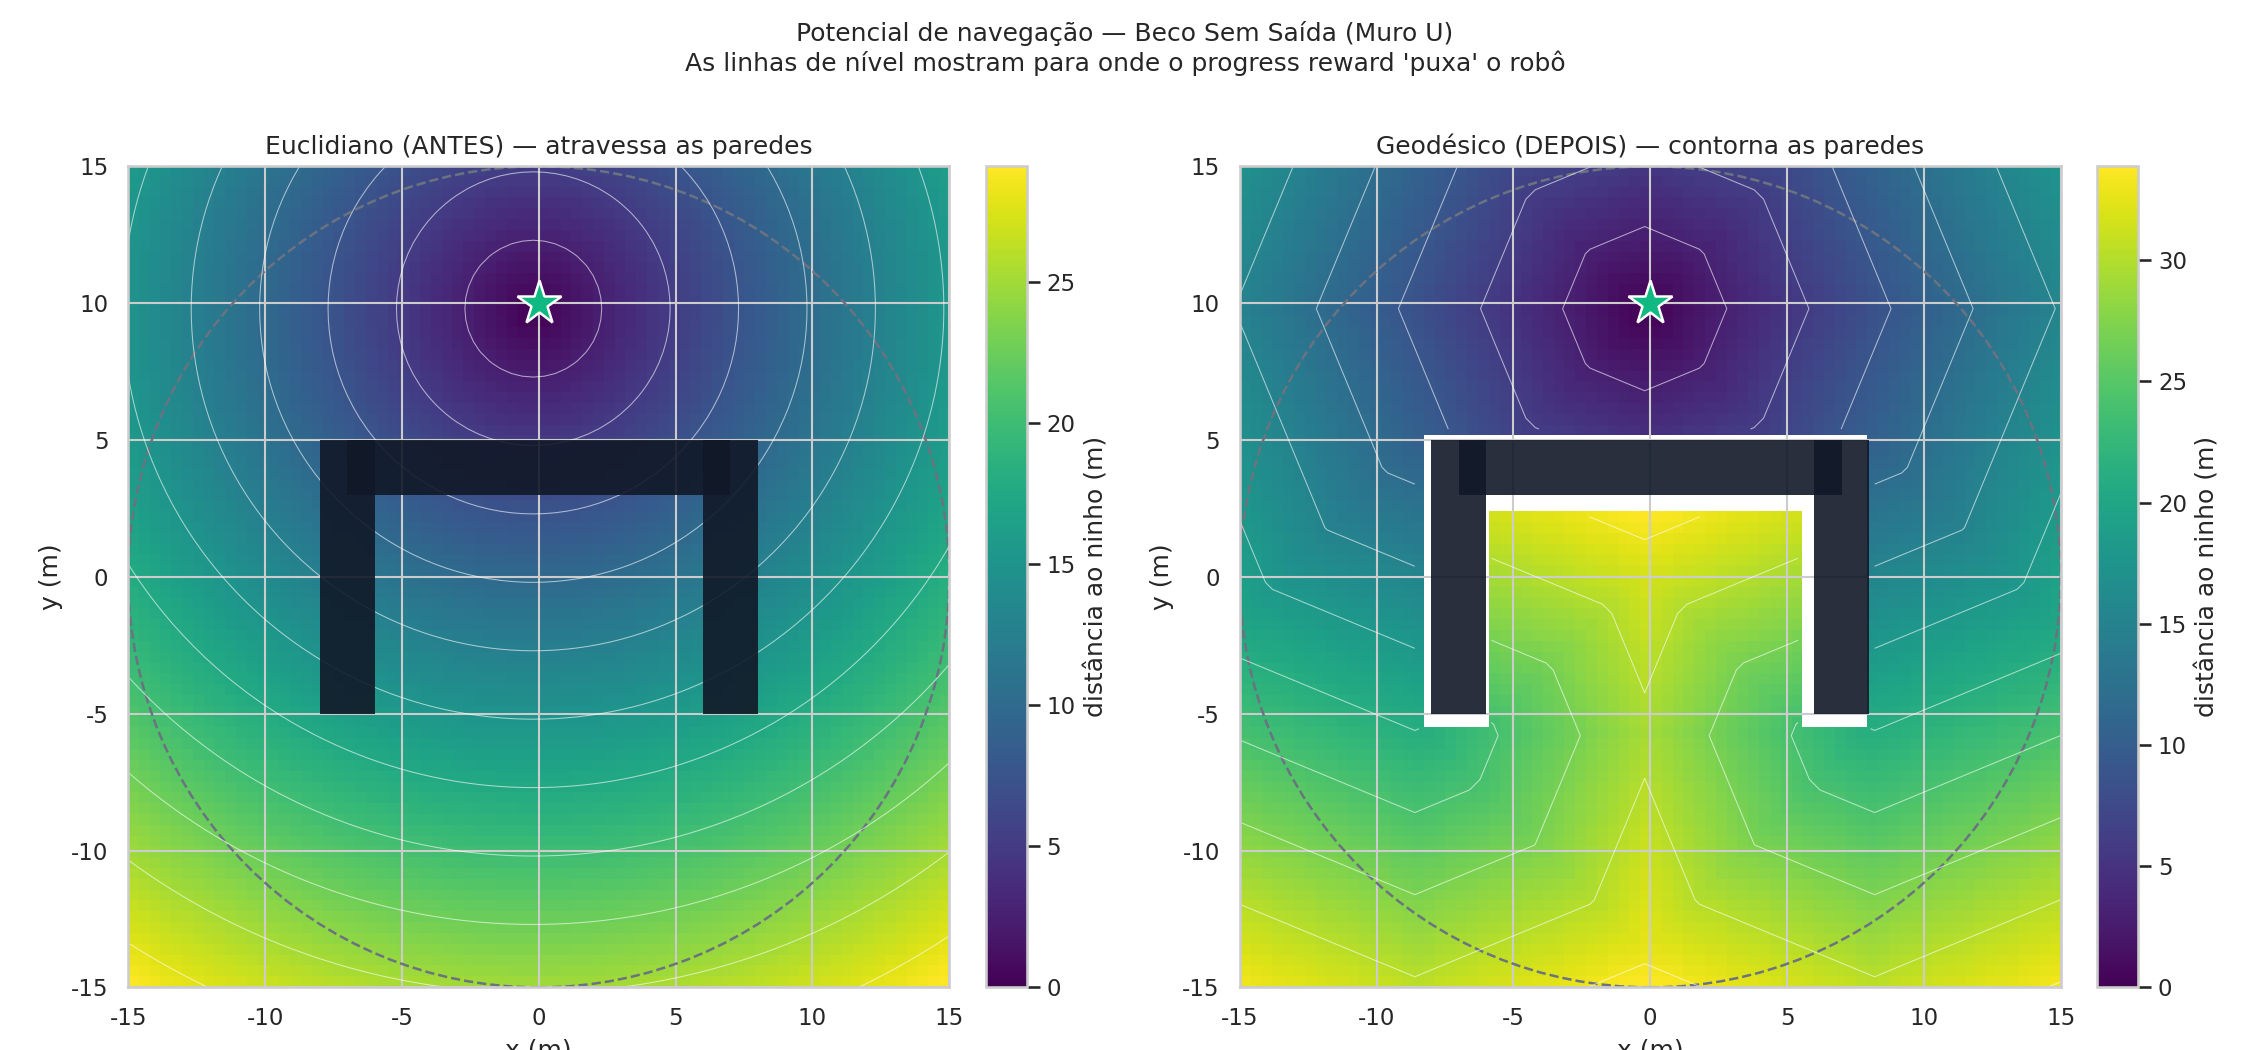
\includegraphics[width=\linewidth]{images/heatmap_geodesico_u_wall.png}
\caption{Potencial de recompensa no Muro em U: a distância euclidiana (esquerda)
atravessa a parede e induz um mínimo local; o campo geodésico (direita), calculado
por Dijkstra sobre a grelha com obstáculos dilatados, premeia o contorno e elimina
a armadilha. É um sinal de treino, não uma observação.}
\label{fig:geodesico}
\end{figure}

\subsection{Espaço de observação, de ação e recompensa}
A observação de cada agente é um vetor egocêntrico que reúne a bússola de
\emph{homing} (direção e distância ao ninho), os oito raios LiDAR e o estado
relativo dos $N-1$ vizinhos; manter o vizinho como uma entidade explícita é o que
permite à GNN atender sobre um conjunto de cardinalidade variável. O espaço de
ação é discreto e egocêntrico: três translações (frente/recuo, esquerda/direita,
cima/baixo) de passo fixo $0.2$\,m, resolvidas por uma ordem determinística de
\emph{step} que aplica deslizamento ao longo das paredes (\emph{wall-sliding}) em
caso de colisão, evitando que o agente fique imobilizado num canto.

A recompensa combina seis termos: (i) uma recompensa esparsa pela entrega de
comida no ninho, que domina; (ii) o progresso geodésico descrito acima
\citep{ng1999policy}; (iii) um bónus de exploração baseado em contagem, que premeia
a visita a novas células e complementa o progresso onde este é plano; (iv) uma
penalização de dispersão que desencoraja a aglomeração em ``bola'', isenta nas
zonas de cooperação para não sabotar a abertura da porta; (v) um custo energético
por passo, que impõe pressão temporal; e (vi) a separação física inter-agente. A
aptidão evolutiva da Equação~\ref{eq:fitness} é, deliberadamente, distinta desta
recompensa: prioriza a comida recolhida e usa o termo modelado apenas como
desempate, ao passo que o PPO/SAC otimizam a recompensa densa completa.

\subsection{Controladores}
O \emph{controlador evolutivo} (GNN) é uma rede compacta que codifica as
características egocêntricas e aplica auto-atenção de produto escalar normalizado
sobre o conjunto de vizinhos \citep{vaswani2017attention}, produzindo uma ação
invariante ao número de vizinhos. Os seus pesos são otimizados por uma estratégia
de evolução $(1{+}\lambda)$ (população $30$, truncatura com elitismo, mutação
gaussiana), com uma aptidão que prioriza a tarefa,
\begin{equation}
J = \bar{f}\cdot 10^4 + 5000\,\tanh\!\left(\bar{R}/5000\right),
\label{eq:fitness}
\end{equation}
onde $\bar{f}$ é a média de comida recolhida e $\bar{R}$ a média da recompensa
modelada; o termo $\tanh$ evita a saturação que, de outro modo, tornaria a seleção
cega (o termo de modelação satura num teto constante e a aptidão deixa de
discriminar genomas). Os \emph{baselines de aprendizagem} são o PPO
\citep{schulman2017ppo} e o SAC \citep{haarnoja2018sac} da biblioteca
Stable-Baselines3, com uma política de perceptrão multicamada partilhada
($[256,256]$) sobre a observação densa da vizinhança (partilha de parâmetros). O
mecanismo de atenção sobre o grafo é, assim, instanciado apenas no controlador
evolutivo, o que é precisamente o que viabiliza a sua transferência
\emph{zero-shot}. O PPO usa estimação de vantagem generalizada
\citep{schulman2016gae} e o SAC, fora de política, regulariza por entropia; ambos
são treinados sobre ambientes vetorizados em paralelo (\emph{SubprocVecEnv}), com
a mesma política a recolher experiência de todos os agentes do enxame, e o
controlador evolutivo avalia a sua população também em paralelo. Para garantir uma
comparação justa, os três controladores partilham o mesmo orçamento de tempo de
treino por cenário e a mesma semente de avaliação.

\subsection{Protocolo de avaliação}
Todos os controladores são avaliados deterministicamente ao longo de $30$
episódios com sementes emparelhadas por cenário. Reportamos $P_{\text{task}}$
(taxa de sucesso, com sucesso definido como pelo menos um item recolhido) e a
média de comida recolhida por episódio, uma métrica comparável entre paradigmas.
A robustez ($R_{\text{robust}}$) injeta a falha de $10\%$ dos agentes a meio do
episódio; a escalabilidade ($S_{\text{scale}}$) testa $N\in\{10,20,50,100\}$ sem
retreino. As diferenças par a par são avaliadas com o teste $U$ de
Mann--Whitney, complementado pelo teste $t$ de Welch, a $\alpha = 0.05$.

\section{Resultados}
\label{sec:results}

\subsection{Desempenho na tarefa}
A Tabela~\ref{tab:task} reporta a comida recolhida por episódio --- a métrica de
magnitude --- a par da taxa de sucesso. Salientamos a primeira: uma taxa de
sucesso de $100\%$ sob a definição ``pelo menos um item recolhido'' é um sinal
fraco, como a tabela deixa claro. Os métodos de gradiente dominam a tarefa: o SAC
recolhe substancialmente nos seis cenários e o PPO em cinco de seis, falhando
apenas o Muro em U, onde recolhe \emph{zero} itens apesar de acumular uma elevada
recompensa modelada --- um caso claro de \emph{exploração da recompensa}, em que o
bónus de exploração é aproveitado sem efetivamente recolher. O controlador
evolutivo é o mais fraco por larga margem: embora ocasionalmente atinja uma taxa
de sucesso não nula (por exemplo, $97\%$ na Perceção Cooperativa), recolhe apenas
quantidades residuais ($2.6$ itens nesse caso, e essencialmente zero nos três
labirintos). Este desfasamento entre uma elevada taxa de sucesso e um rendimento
quase nulo é a assinatura da \emph{exploração da aptidão}: a aptidão de treino
sobe sem se traduzir em conclusão da tarefa. A
Figura~\ref{fig:recolhas} visualiza estas diferenças de magnitude.

\begin{table*}[t]
\centering
\caption{Desempenho por episódio sob avaliação determinística ($30$ episódios com
sementes emparelhadas por cenário, execução oficial): média de comida recolhida
$\pm$ desvio-padrão, com a taxa de sucesso (percentagem de episódios com pelo
menos um item recolhido) entre parênteses. A comida recolhida é a métrica de
magnitude comparada entre paradigmas; a taxa de sucesso, isolada, é um indicador
fraco, pois um agente atinge $100\%$ recolhendo um único item. Melhor média por
linha a negrito.}
\label{tab:task}
\footnotesize
\begin{tabular}{lccc}
\toprule
Cenário & GNN & PPO & SAC \\
\midrule
Sandbox                & $0.8\pm0.7$ (67\%) & $\mathbf{73.3\pm5.1}$ (100\%) & $25.2\pm3.6$ (100\%) \\
Muro em U              & $0.4\pm0.5$ (43\%) & $0.0\pm0.0$ (0\%)            & $\mathbf{20.6\pm1.3}$ (100\%) \\
Gargalo                & $0.0\pm0.0$ (0\%)  & $\mathbf{41.0\pm1.4}$ (100\%) & $35.0\pm1.6$ (100\%) \\
Quatro Salas           & $0.0\pm0.0$ (0\%)  & $11.5\pm3.4$ (100\%)        & $\mathbf{11.6\pm3.0}$ (100\%) \\
Porta Cooperativa      & $0.0\pm0.0$ (0\%)  & $\mathbf{67.7\pm1.6}$ (100\%) & $60.5\pm1.3$ (100\%) \\
Perceção Cooperativa   & $2.6\pm1.4$ (97\%) & $\mathbf{17.9\pm1.9}$ (100\%) & $16.2\pm1.8$ (100\%) \\
\bottomrule
\end{tabular}
\end{table*}

\begin{figure}[t]
\centering
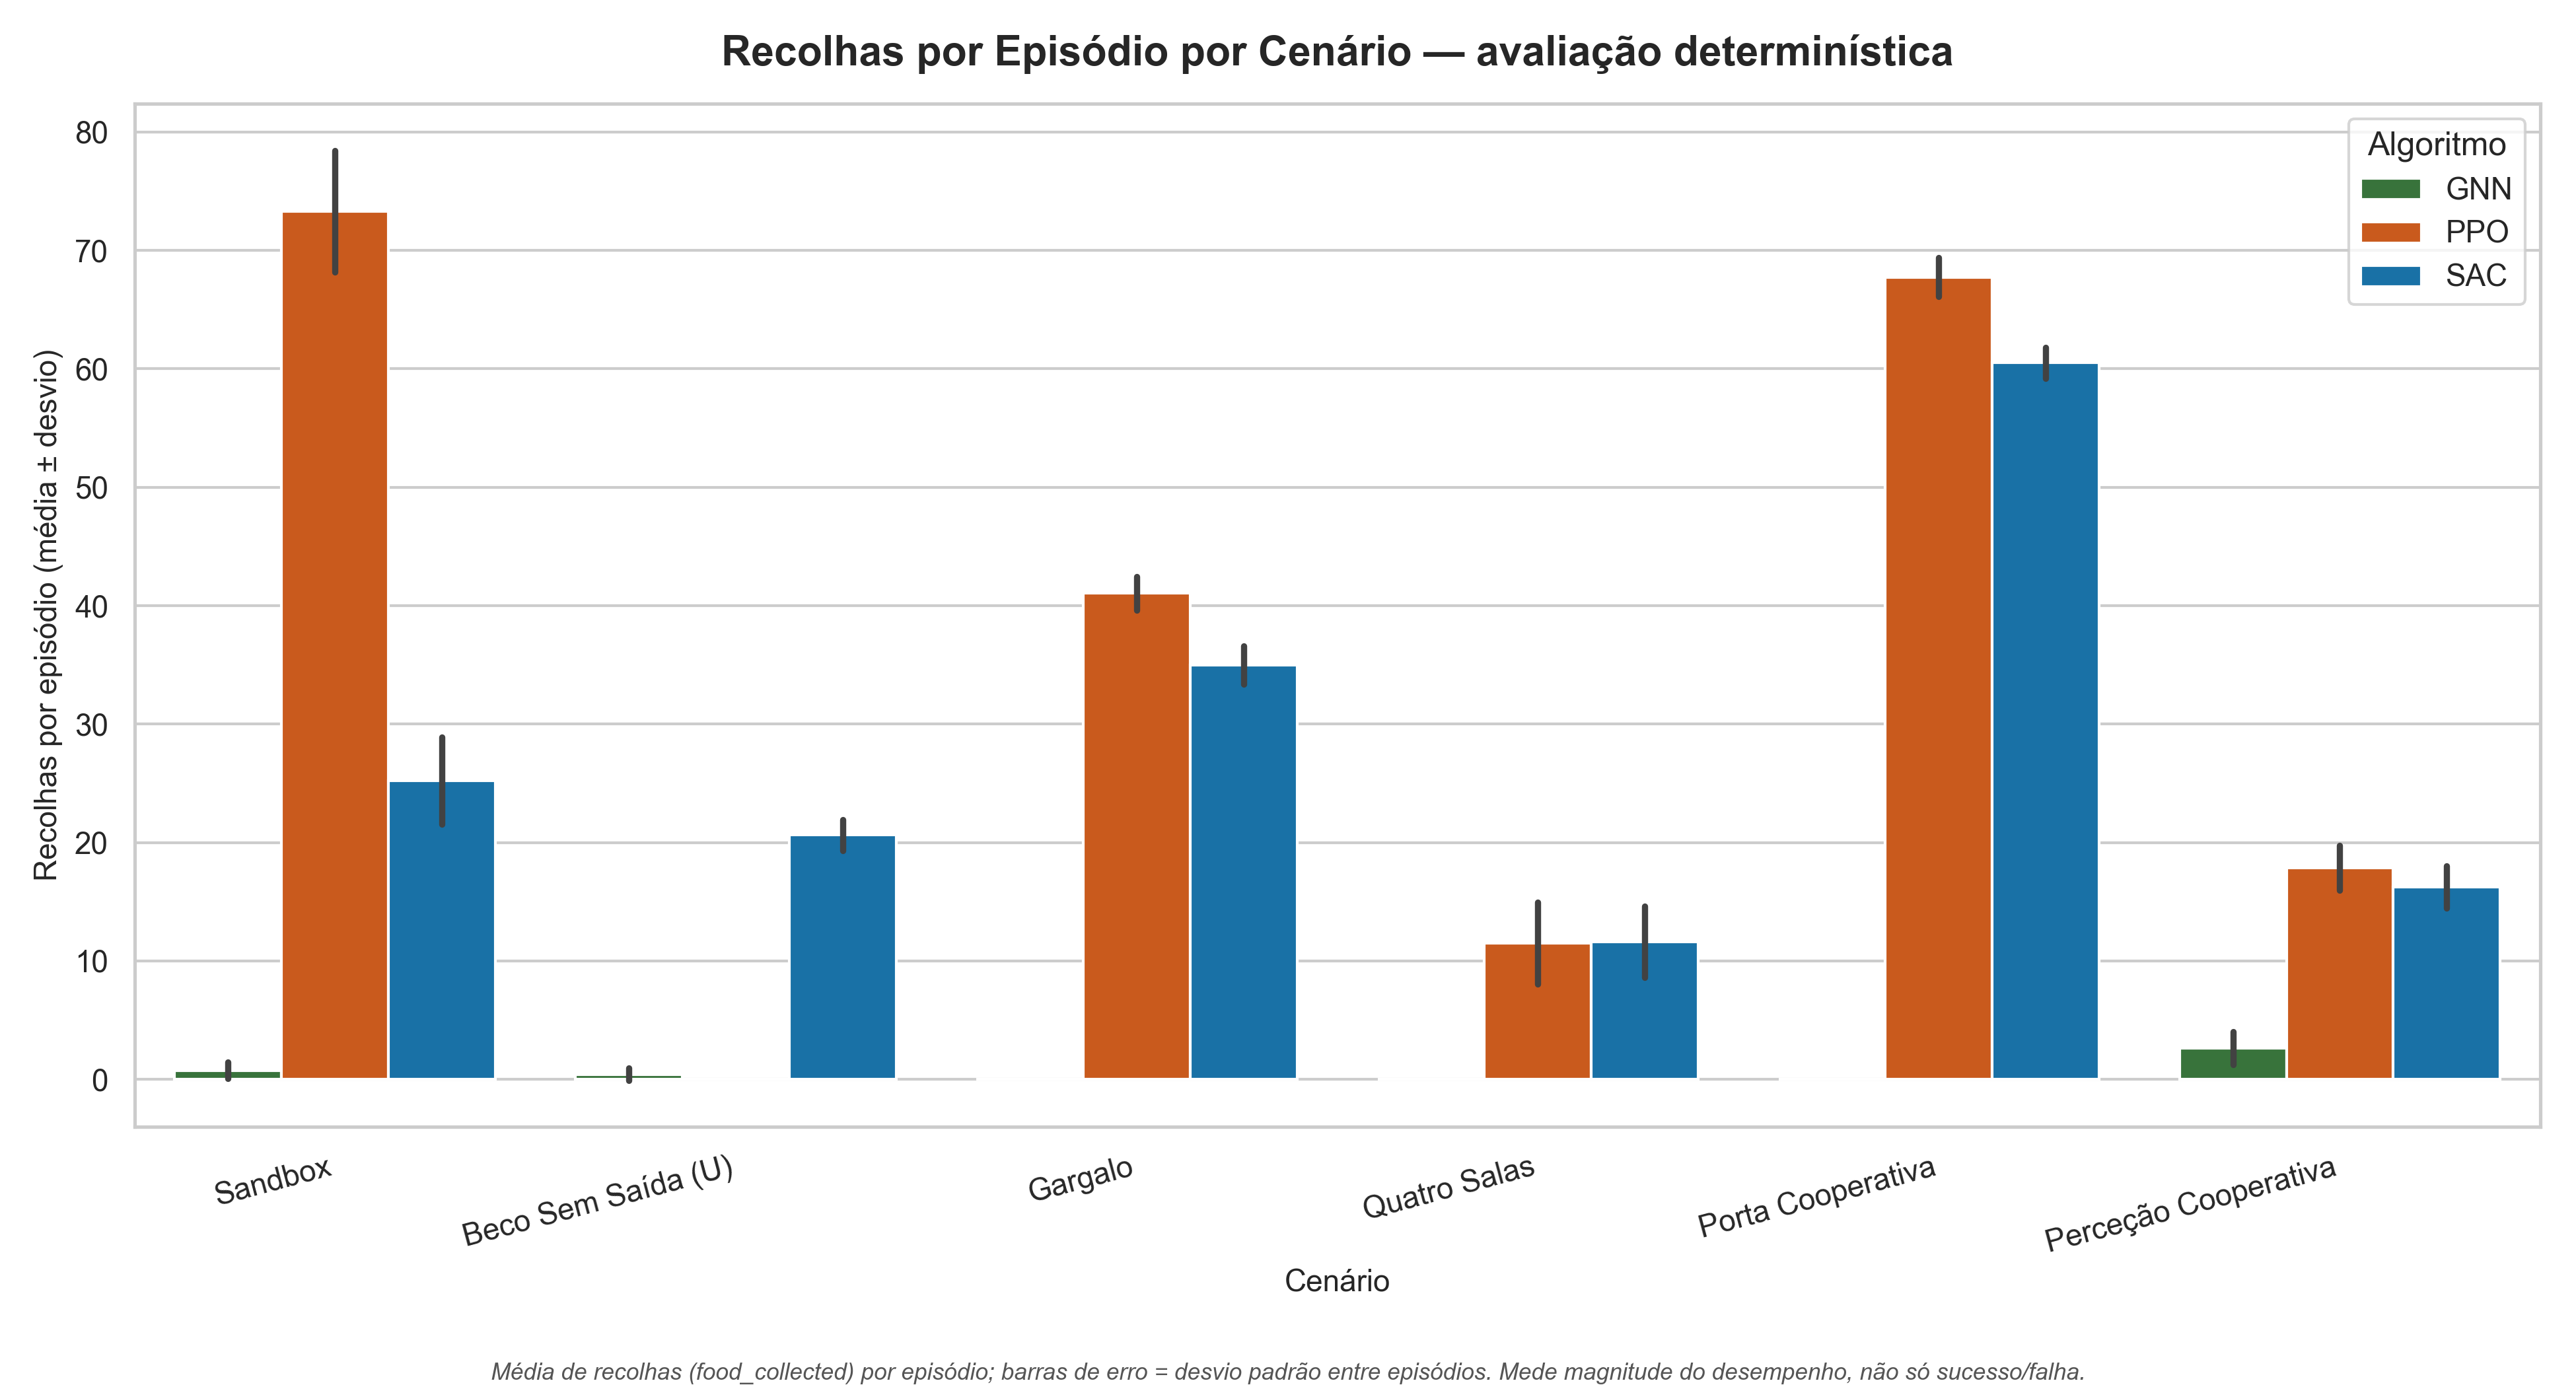
\includegraphics[width=\linewidth]{images/recolhas_por_cenario.png}
\caption{Comida recolhida por episódio (média $\pm$ desvio-padrão) por cenário e
controlador. O contraste de magnitude entre os métodos de gradiente e o
controlador evolutivo é evidente, mesmo onde este último regista sucesso
não nulo.}
\label{fig:recolhas}
\end{figure}

\subsection{Análise qualitativa da navegação}
Os mapas de ocupação acumulada explicam \emph{como} cada controlador se comporta
no Muro em U (Figura~\ref{fig:ocupacao}). O controlador evolutivo fica preso
abaixo da barra e nunca alcança o ninho; o PPO espalha-se pela arena a colher o
bónus de exploração mas sem completar a entrega --- a marca visual do
\emph{reward hacking}, em que a recompensa modelada sobe sem produzir comida; e o
SAC contorna o muro pelos dois lados e converge para o ninho. A diferença não é de
perceção --- os três partilham a mesma observação --- mas de qualidade da política
aprendida sob a mesma recompensa geodésica.

\begin{figure*}[t]
\centering
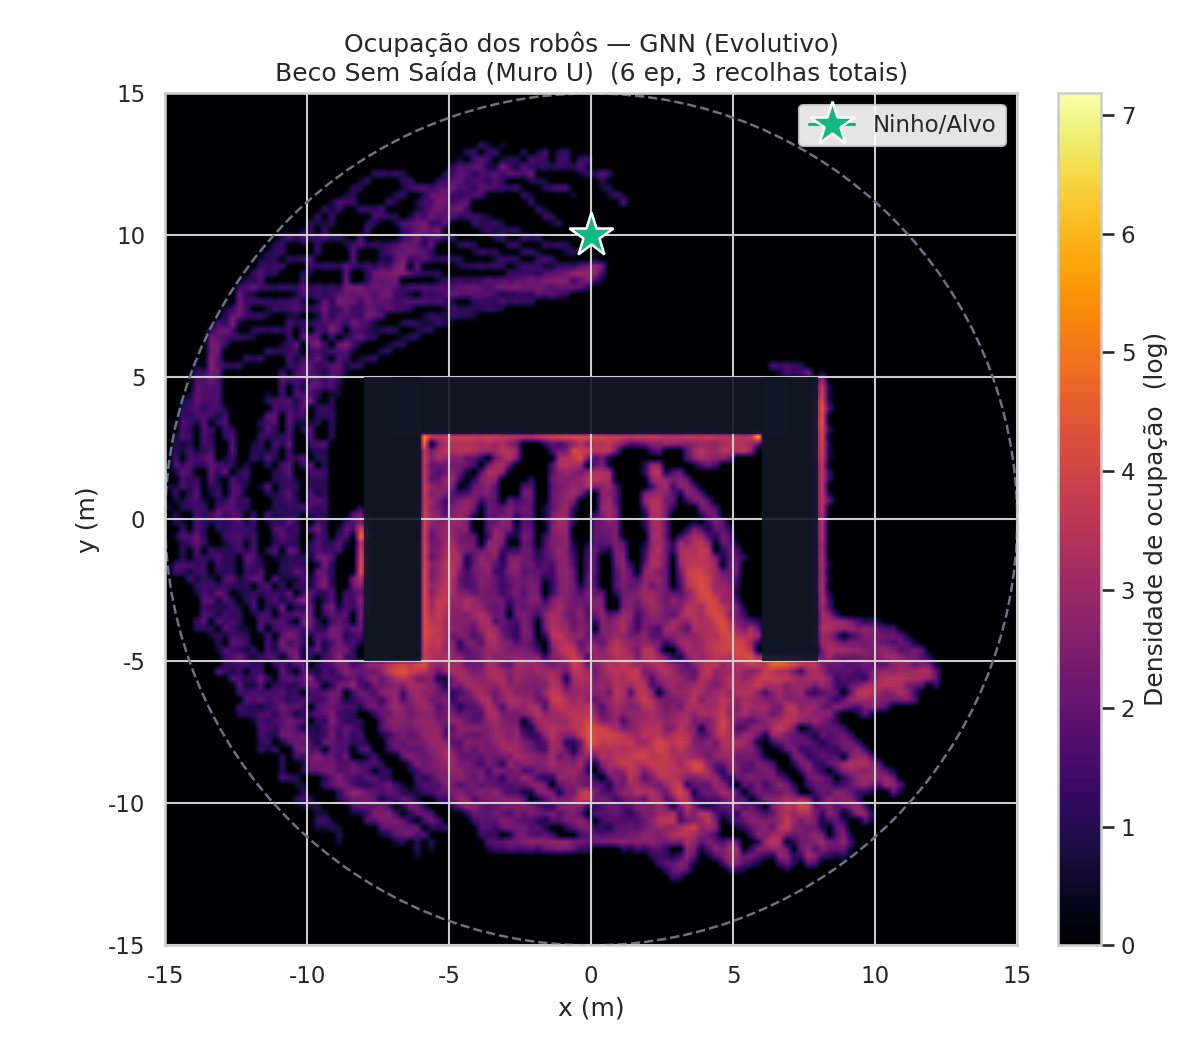
\includegraphics[width=0.32\linewidth]{images/heatmap_ocupacao_gnn_u_wall.png}\hfill
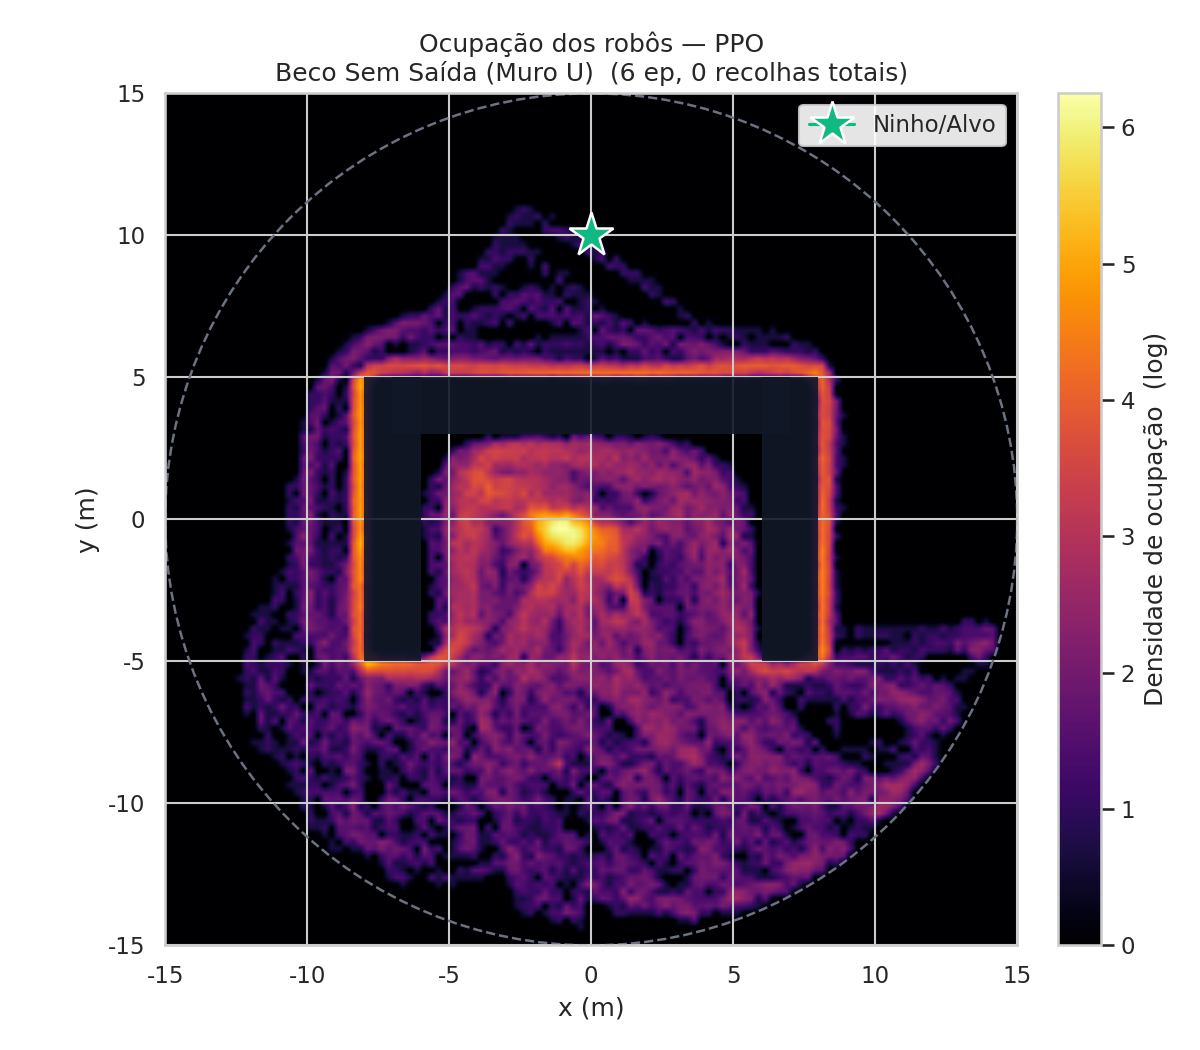
\includegraphics[width=0.32\linewidth]{images/heatmap_ocupacao_ppo_u_wall.png}\hfill
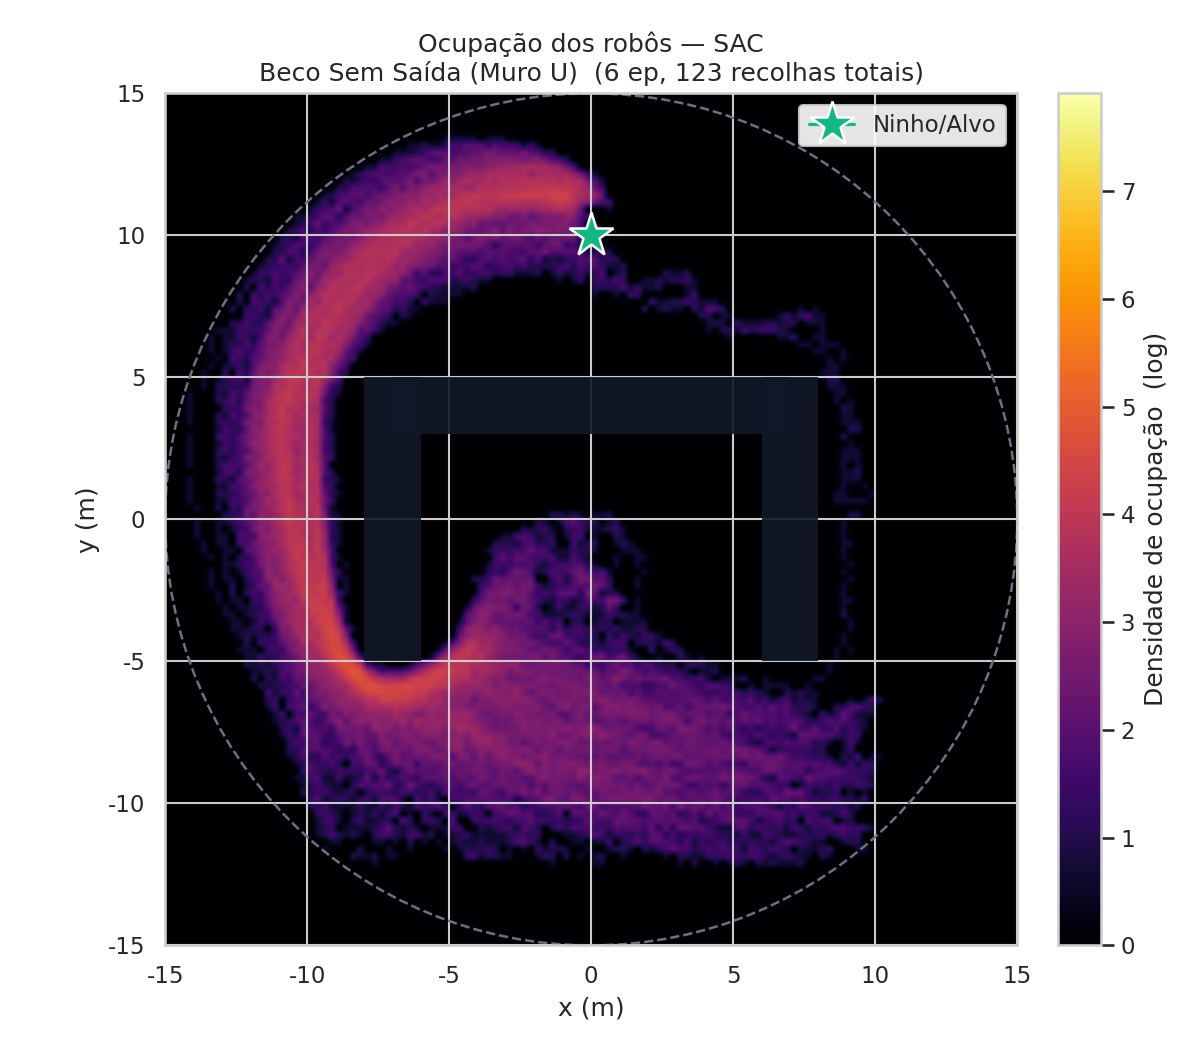
\includegraphics[width=0.32\linewidth]{images/heatmap_ocupacao_sac_u_wall.png}
\caption{Mapas de ocupação no Muro em U (escala logarítmica). O controlador
evolutivo (esquerda) fica preso abaixo da barra; o PPO (centro) percorre a arena a
explorar mas sem entregar comida (\emph{reward hacking}); o SAC (direita)
contorna o muro pelos dois lados e atinge o ninho. Mesma observação, políticas
distintas.}
\label{fig:ocupacao}
\end{figure*}

\subsection{Escalabilidade \emph{zero-shot}}
O compromisso emerge sob a escalabilidade. Apenas o controlador baseado em atenção
é viável para $N\neq 20$: a sua taxa de sucesso \emph{aumenta} com o tamanho do
enxame, de $15\%$ em $N=10$ para $100\%$ em $N=100$, sem degradação per capita
(Figura~\ref{fig:escala}). As políticas de perceptrão multicamada do PPO/SAC têm
uma entrada de dimensão fixa e são estruturalmente incompatíveis com outros
tamanhos de enxame. A adaptabilidade arquitetural --- a propriedade que a hipótese
atribui ao MARL --- manifesta-se, assim, na \emph{representação} (grafo com
atenção), e não no algoritmo de otimização.

\begin{figure}[t]
\centering
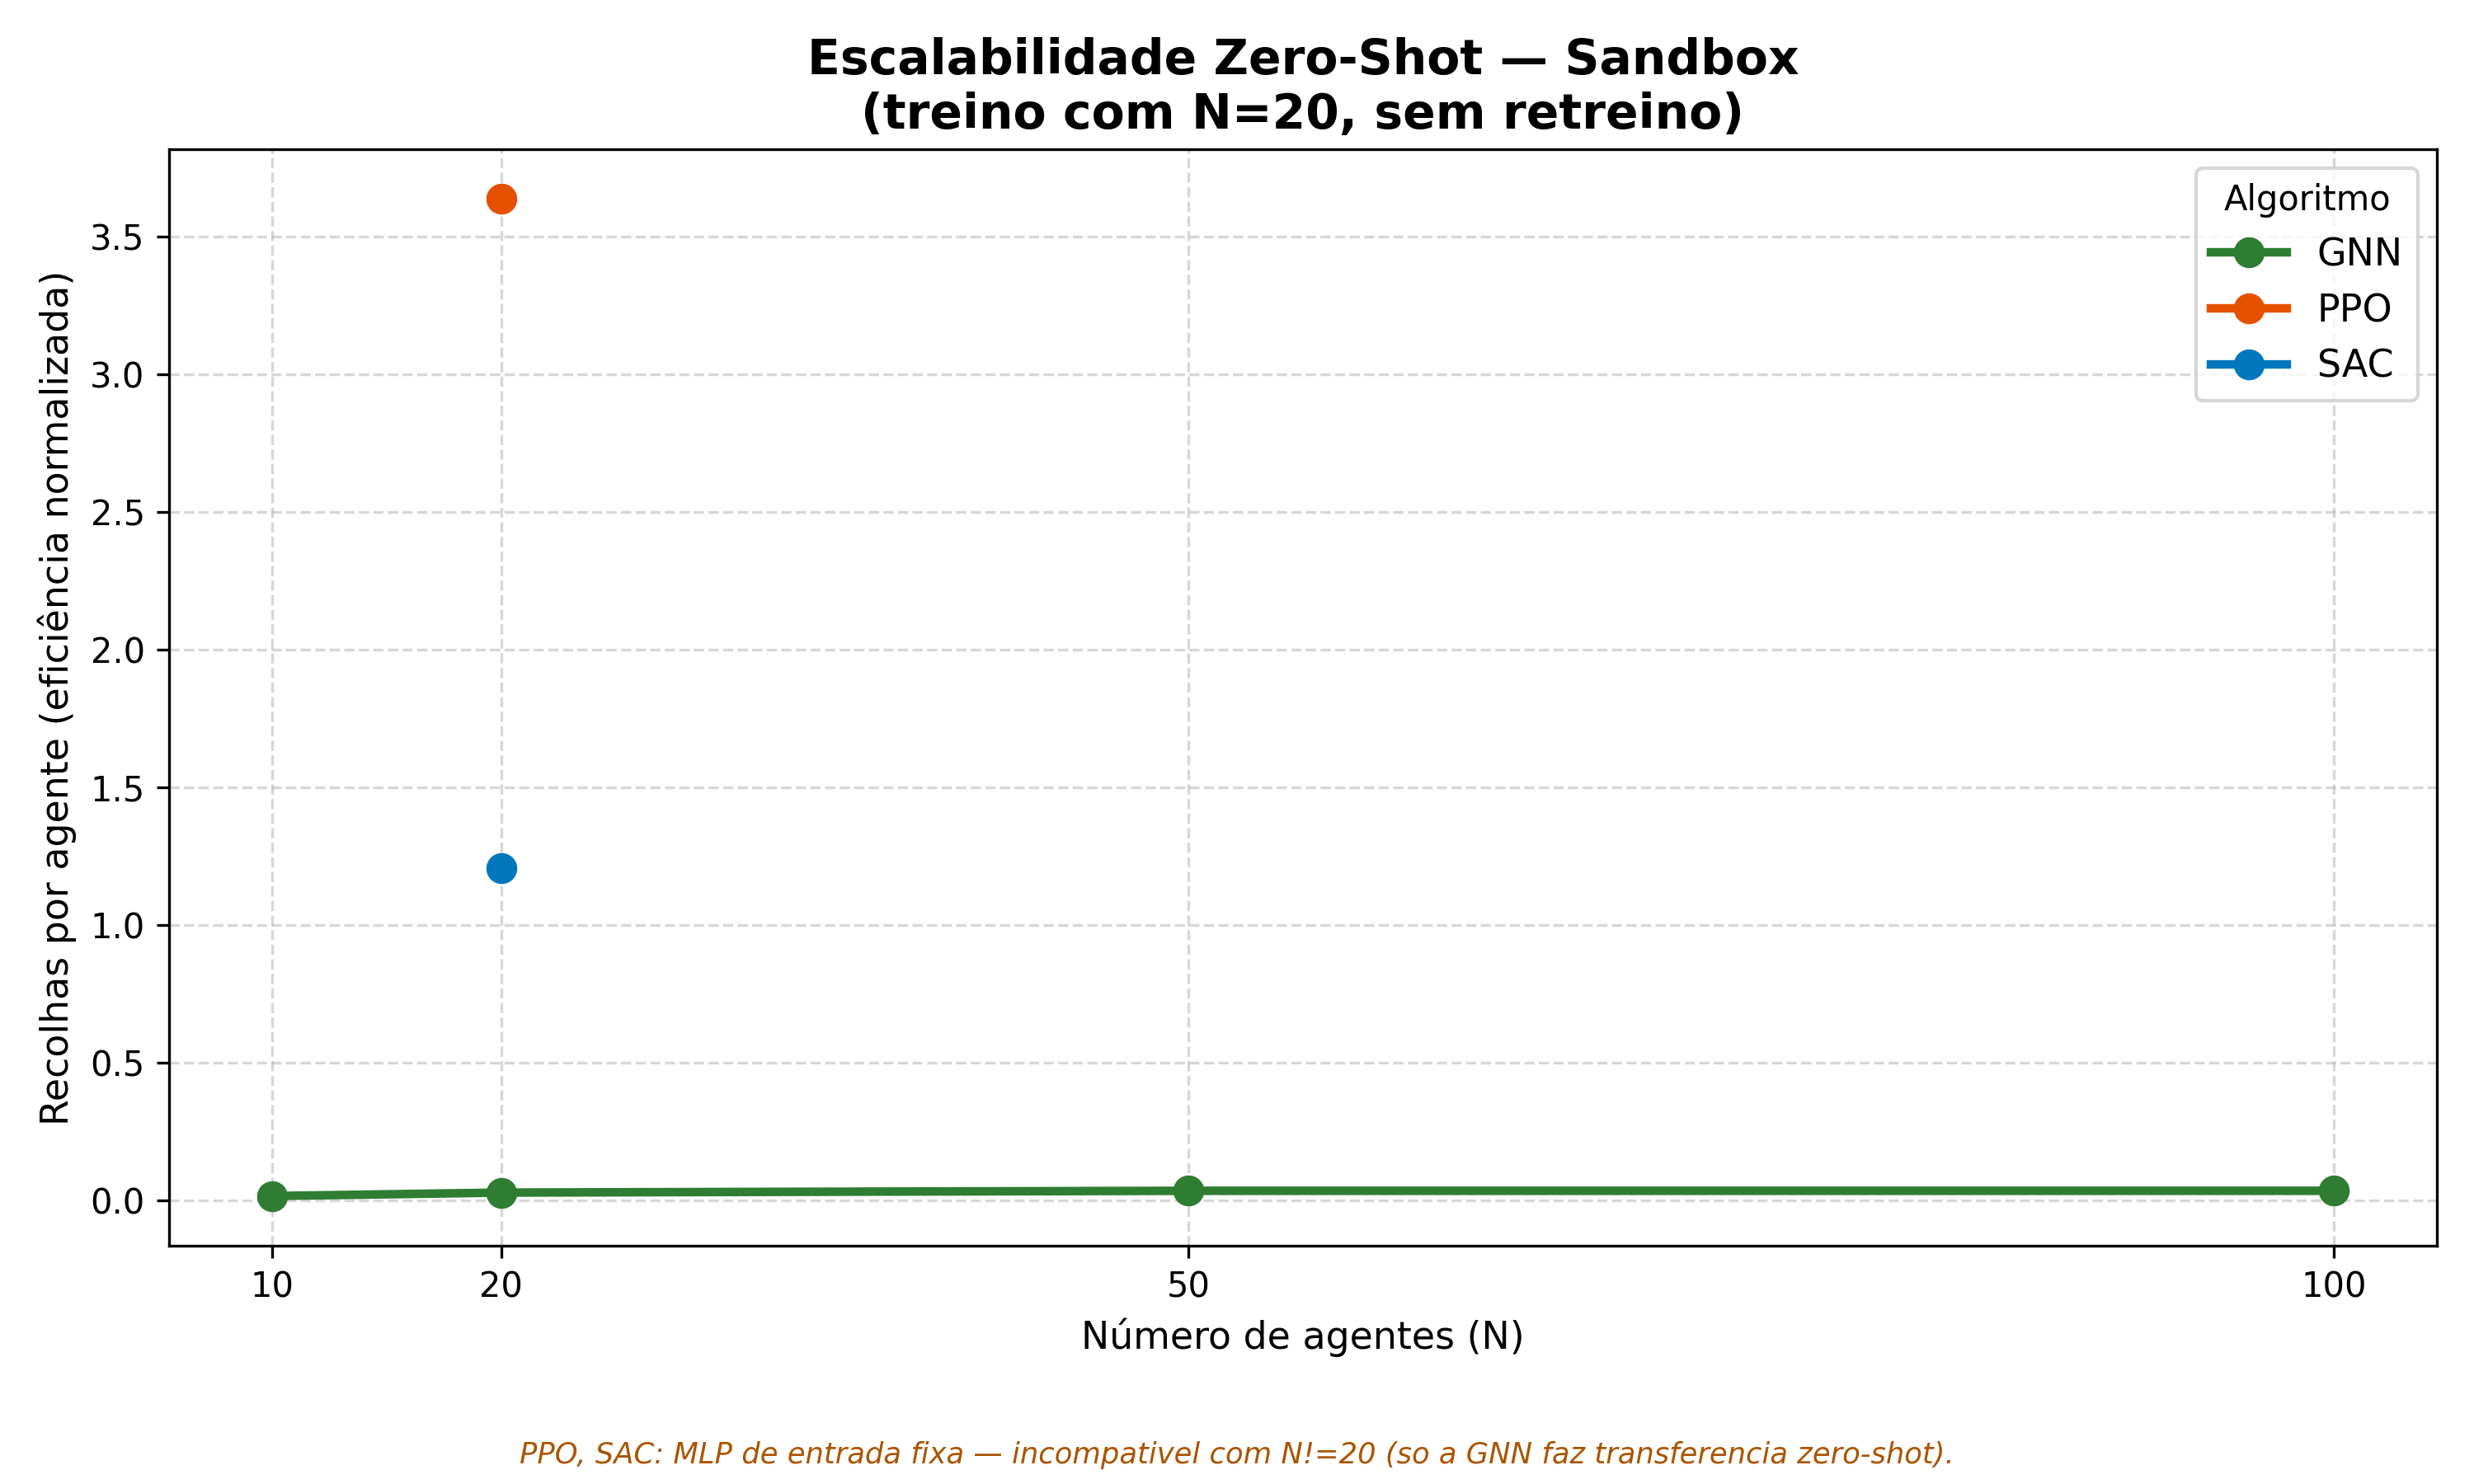
\includegraphics[width=\linewidth]{images/escalabilidade_zeroshot_none.png}
\caption{Transferência \emph{zero-shot} para tamanhos de enxame nunca vistos
($N\in\{10,20,50,100\}$), sem retreino. Só o controlador com atenção sobre o grafo
é estruturalmente compatível com $N\neq 20$, e a sua taxa de sucesso melhora com o
tamanho do enxame. O PPO/SAC, com entrada de dimensão fixa, são incompatíveis.}
\label{fig:escala}
\end{figure}

\subsection{Robustez}
Sob a falha de $10\%$ dos agentes a meio do episódio, todos os paradigmas mantêm
desempenho elevado ($94$--$99\%$ dos itens recolhidos para o PPO/SAC; $69$--$96\%$
para o GNN onde funciona), sem colapso (Figura~\ref{fig:robustez}): a partilha de
parâmetros e a observação local conferem redundância funcional ao enxame.

\begin{figure}[t]
\centering
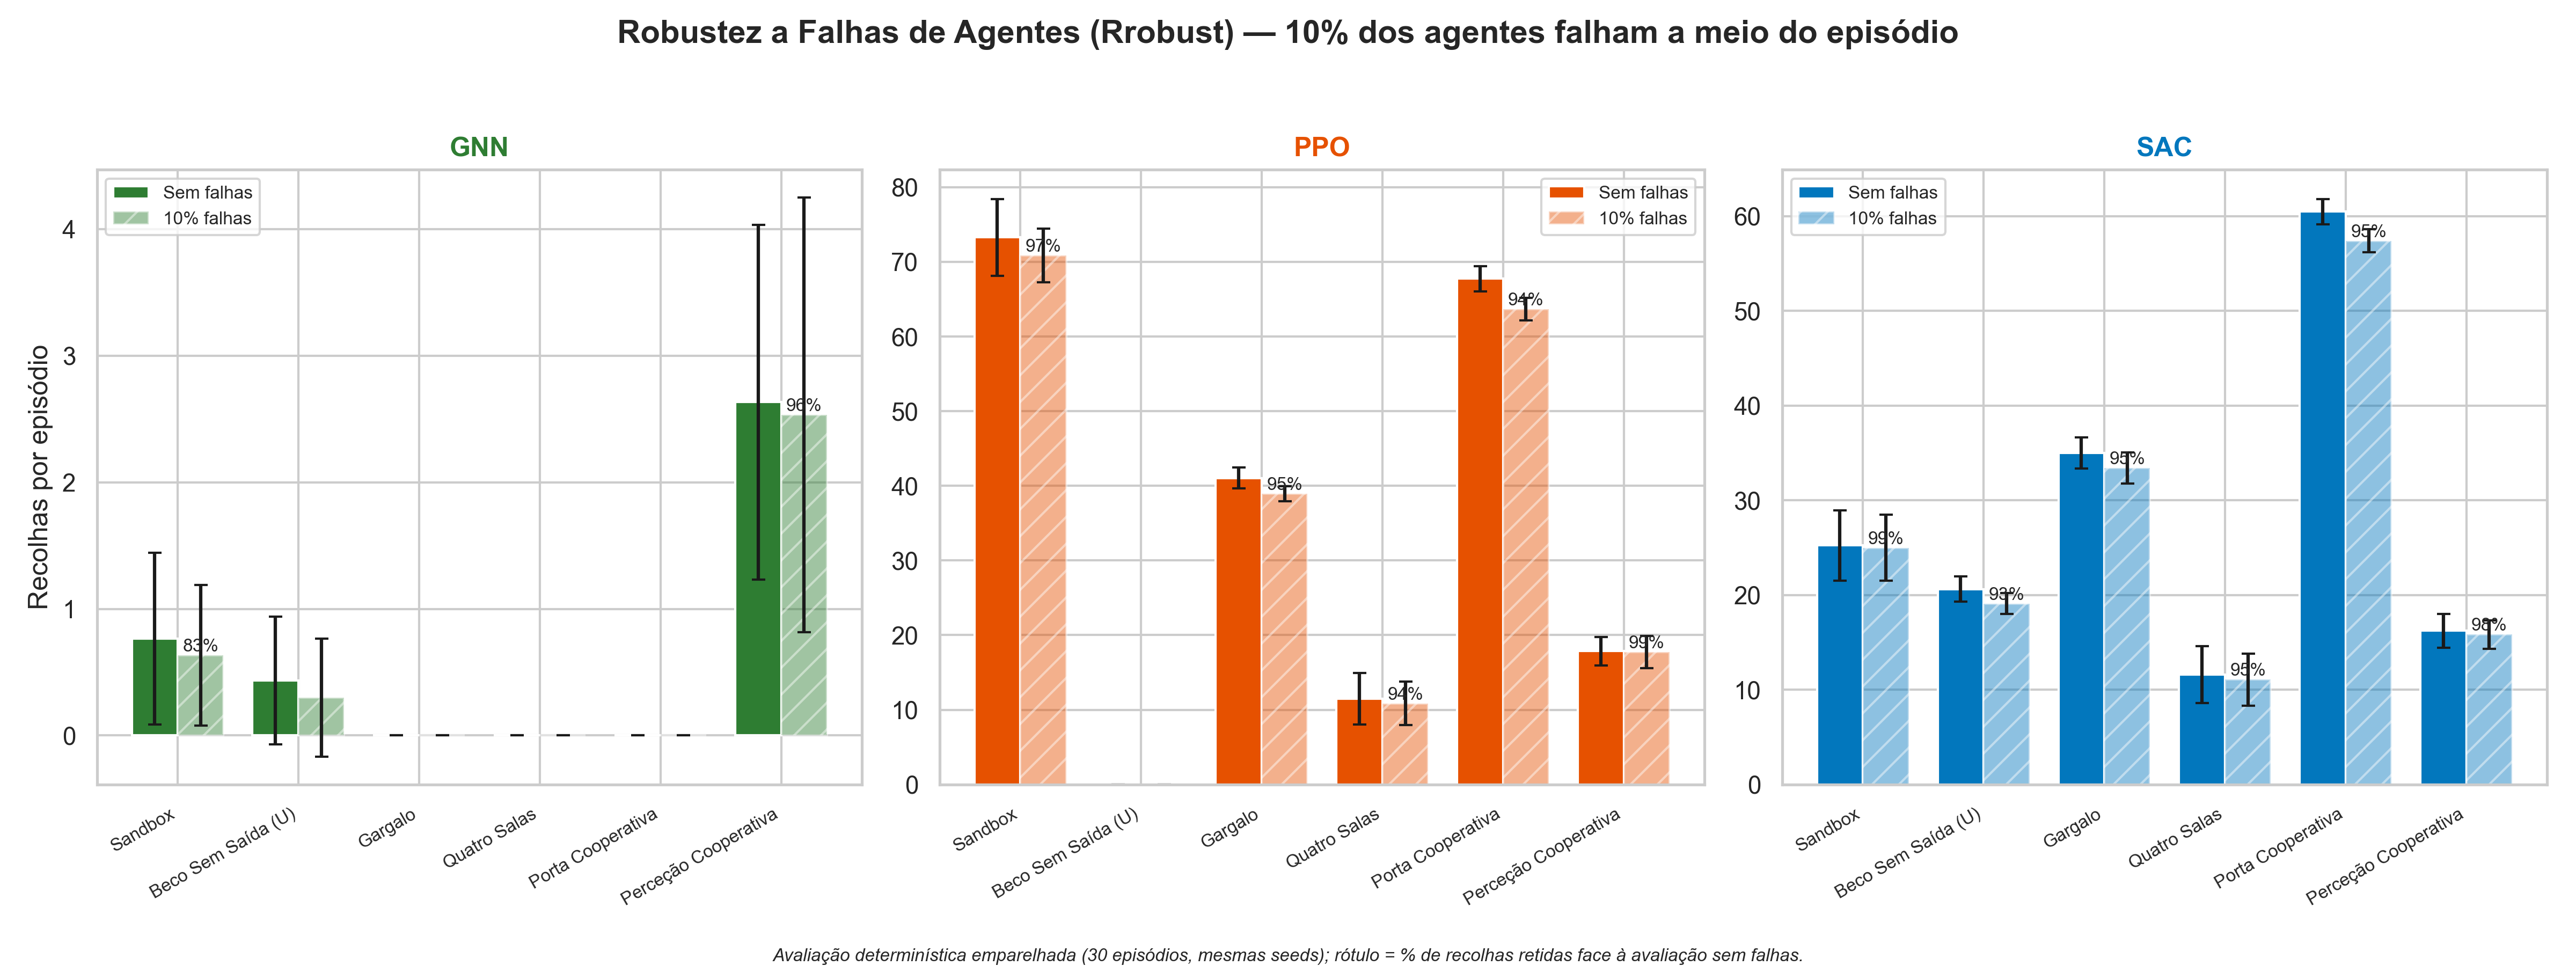
\includegraphics[width=\linewidth]{images/robustez_falhas.png}
\caption{Retenção de desempenho sob falha de $10\%$ dos agentes a meio do
episódio, relativa à execução nominal. Nenhum paradigma colapsa; a redundância
emerge da partilha de parâmetros e da observação puramente local.}
\label{fig:robustez}
\end{figure}

\subsection{Significância estatística}
A Tabela~\ref{tab:signif} apresenta as $18$ comparações par a par sobre a comida
recolhida. Dezassete são significativas ($p<0.001$); a única exceção é PPO vs.\
SAC nas Quatro Salas ($p=0.53$), onde os dois métodos de gradiente são
estatisticamente indistinguíveis. A magnitude e a consistência destas diferenças
confirmam que o ordenamento dos controladores não é um artefacto da variância
amostral.

\begin{table*}[t]
\centering
\caption{Testes de significância sobre a comida recolhida ($30$ episódios
emparelhados; teste $U$ de Mann--Whitney, $\alpha=0.05$). ``méd.~A'' e ``méd.~B''
são as médias de comida recolhida de cada elemento do par.}
\label{tab:signif}
\footnotesize
\begin{tabular}{llrrrl}
\toprule
Cenário & Par & méd.~A & méd.~B & $p$ & Significativo \\
\midrule
Sandbox              & GNN vs PPO & 0.77 & 73.30 & $<0.001$ & Sim \\
Sandbox              & GNN vs SAC & 0.77 & 25.23 & $<0.001$ & Sim \\
Sandbox              & PPO vs SAC & 73.30 & 25.23 & $<0.001$ & Sim \\
Muro em U            & GNN vs PPO & 0.43 & 0.00 & $0.0003$ & Sim \\
Muro em U            & GNN vs SAC & 0.43 & 20.63 & $<0.001$ & Sim \\
Muro em U            & PPO vs SAC & 0.00 & 20.63 & $<0.001$ & Sim \\
Gargalo              & GNN vs PPO & 0.00 & 41.03 & $<0.001$ & Sim \\
Gargalo              & GNN vs SAC & 0.00 & 35.00 & $<0.001$ & Sim \\
Gargalo              & PPO vs SAC & 41.03 & 35.00 & $<0.001$ & Sim \\
Quatro Salas         & GNN vs PPO & 0.00 & 11.50 & $<0.001$ & Sim \\
Quatro Salas         & GNN vs SAC & 0.00 & 11.60 & $<0.001$ & Sim \\
Quatro Salas         & PPO vs SAC & 11.50 & 11.60 & $0.5312$ & não \\
Porta Cooperativa    & GNN vs PPO & 0.00 & 67.73 & $<0.001$ & Sim \\
Porta Cooperativa    & GNN vs SAC & 0.00 & 60.50 & $<0.001$ & Sim \\
Porta Cooperativa    & PPO vs SAC & 67.73 & 60.50 & $<0.001$ & Sim \\
Perceção Cooperativa & GNN vs PPO & 2.63 & 17.87 & $<0.001$ & Sim \\
Perceção Cooperativa & GNN vs SAC & 2.63 & 16.23 & $<0.001$ & Sim \\
Perceção Cooperativa & PPO vs SAC & 17.87 & 16.23 & $<0.001$ & Sim \\
\bottomrule
\end{tabular}
\end{table*}

\section{Discussão}
\label{sec:discussion}
O colapso do controlador evolutivo nos cenários de labirinto não é uma
propriedade da arquitetura --- a mesma representação de grafo com atenção sustenta
a sua vantagem de escalabilidade --- mas da interação entre o método de otimização
e a estrutura da recompensa. A neuroevolução otimiza a partir de um único escalar
de aptidão por episódio, sem atribuição de crédito temporal; nunca aprende
\emph{qual} ação importou. Quando a recompensa de tarefa é esparsa, como nos
labirintos, quase todos os genomas não recolhem comida, a aptidão reduz-se ao
termo de modelação (saturado) e a população instala-se num \emph{planalto de
aptidão} onde a pressão seletiva desaparece. A mesma natureza estocástica explica
a elevada variância entre execuções independentes, ausente nos métodos de
gradiente: sem um gradiente a puxar cada execução para um ótimo comum, cada
execução é um passeio aleatório distinto sobre a paisagem de aptidão, e encontrar
o vale estreito das soluções dos labirintos depende largamente do número de
gerações exploradas.

Decorrem duas implicações. Primeira, a comparação combina dois fatores ---
algoritmo de otimização e arquitetura de rede --- pelo que a limitação observada é
de \emph{eficiência amostral} do otimizador, e não de capacidade representacional;
integrar o módulo de atenção numa política treinada por gradiente é o passo
natural para isolar o efeito. Segunda, o valor de engenharia não está em eleger um
vencedor, mas em identificar o ponto de inflexão: a escolha do paradigma deve
seguir o eixo de exigência dominante --- desempenho na tarefa a um tamanho de
enxame fixo (MARL) \emph{versus} escalabilidade para tamanhos nunca vistos (grafo
com atenção).

\section{Limitações do estudo}
\label{sec:limitacoes}
Três limitações enquadram o alcance das conclusões. Primeira, e mais importante, a
comparação é \emph{assimétrica}: o controlador evolutivo usa uma arquitetura de
grafo com atenção, enquanto os \emph{baselines} de gradiente usam um perceptrão
multicamada de entrada fixa. Isolar o efeito do otimizador exigiria treinar a
mesma arquitetura de atenção por gradiente --- o passo natural já identificado.
Segunda, os números determinísticos reportados resultam de uma execução de treino
oficial por controlador; embora a avaliação use $30$ episódios com sementes
emparelhadas, a variância \emph{entre} execuções de treino da neuroevolução é
elevada e só um protocolo de execução múltipla a poderá quantificar plenamente.
Terceira, todos os resultados são em simulação; a transferência para hardware real
introduz o conhecido \emph{reality gap}, cuja mitigação por aleatorização de
domínio \citep{tobin2017domain} fica como trabalho futuro. Estas limitações não
invalidam o achado central --- o compromisso desempenho/escalabilidade é robusto e
estatisticamente suportado --- mas delimitam-no com honestidade.

\section{Conclusões}
\label{sec:conclusions}
Apresentámos uma avaliação comparativa imparcial de um controlador de atenção
neuroevoluído contra o PPO e o SAC num enxame de \emph{foraging} tridimensional,
ao longo de seis cenários e três eixos de avaliação com suporte estatístico. A
hipótese de que a inteligência adaptativa domina a robustez estática é apenas
parcialmente confirmada: os métodos de gradiente vencem decisivamente na conclusão
da tarefa a $N=20$, enquanto apenas o controlador baseado em atenção escala
\emph{zero-shot} até $N=100$. O trabalho futuro inclui uma política de atenção
treinada por gradiente para separar o otimizador da arquitetura, um protocolo de
execução múltipla para consolidar as estimativas de variância, e a validação da
transferência simulação-para-real \citep{tobin2017domain}.

\section*{Agradecimentos}
Este artigo foi parcialmente financiado por fundos nacionais através da Funda\c{c}\~ao
para a Ci\^encia e a Tecnologia, I.P. (FCT), Projetos Plurianuais ISTAR-Iscte
UID/04466/2025 (\url{https://doi.org/10.54499/UID/04466/2025}).

\bibliographystyle{elsarticle-harv}
\bibliography{references}

\end{document}
